% Auto-generado por phase2/build_appendix_montages.py — no editar a mano.
% Regenerar tras nuevas reconstrucciones y volver a compilar.
% Layout: 2 tira(s) por hoja (doble columna comprimida).

\begin{figure}[htbp]
  \centering
  \begin{minipage}[t]{0.49\textwidth}
    \centering
    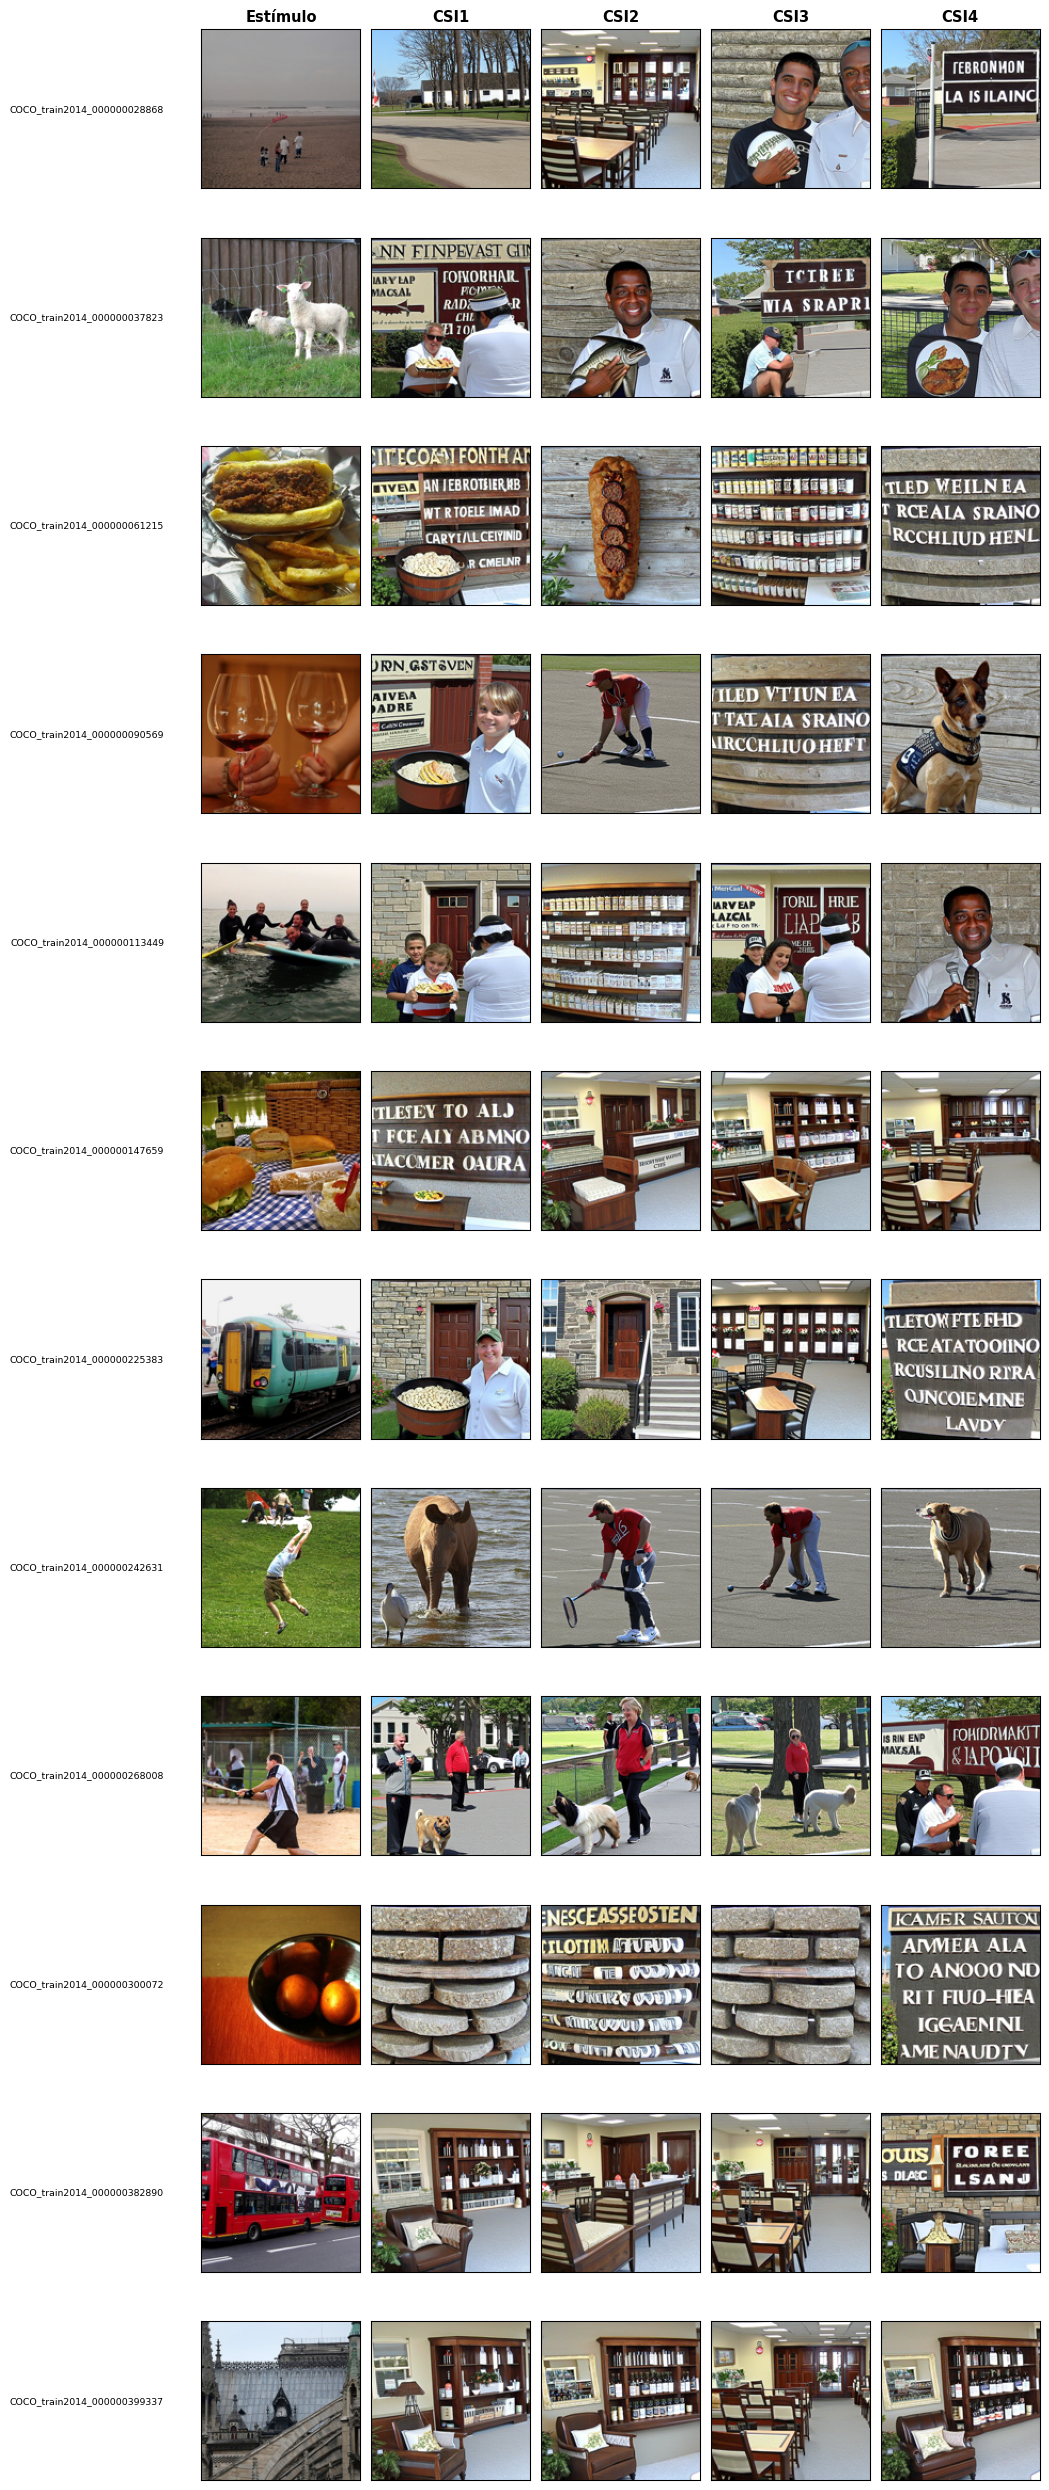
\includegraphics[width=\linewidth]{Figures/reconstrucciones/apendice/apendiceB_galeria_p01.png}
  \end{minipage}  \hfill
  \begin{minipage}[t]{0.49\textwidth}
    \centering
    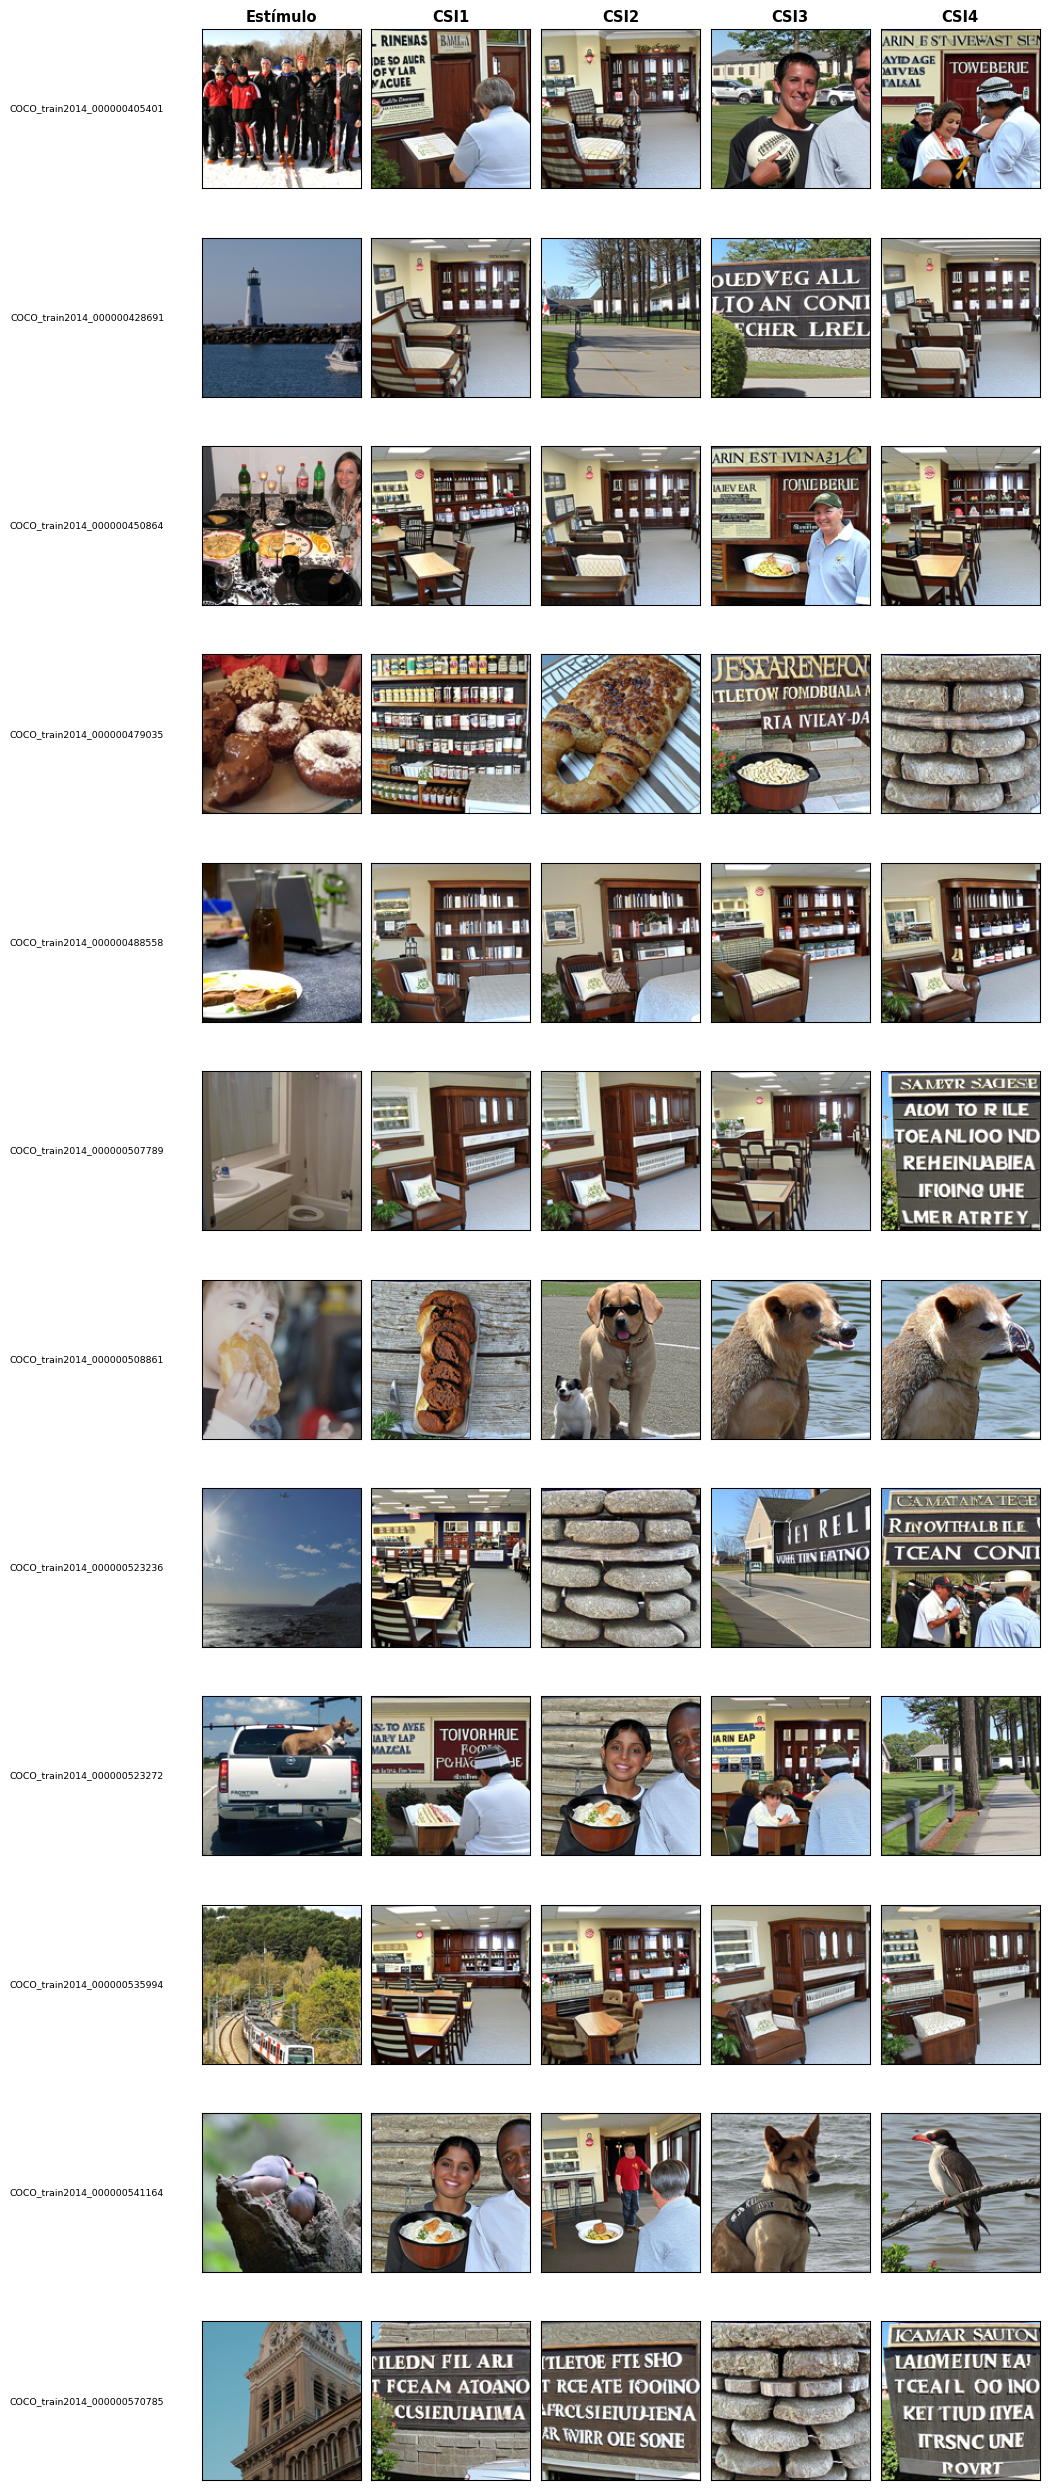
\includegraphics[width=\linewidth]{Figures/reconstrucciones/apendice/apendiceB_galeria_p02.png}
  \end{minipage}
  \caption[Galería de reconstrucciones (partes 1--2/5)]{Reconstrucciones cross-subject sobre estímulos BOLD5000 (partes 1--2 de 5). Columna~1: estímulo original; columnas~2--5: reconstrucción SD~2.1 unCLIP por sujeto (CSI1, CSI2, CSI3, CSI4).}
  \label{fig:apendiceB_galeria:g01}
\end{figure}
\clearpage

\begin{figure}[htbp]
  \centering
  \begin{minipage}[t]{0.49\textwidth}
    \centering
    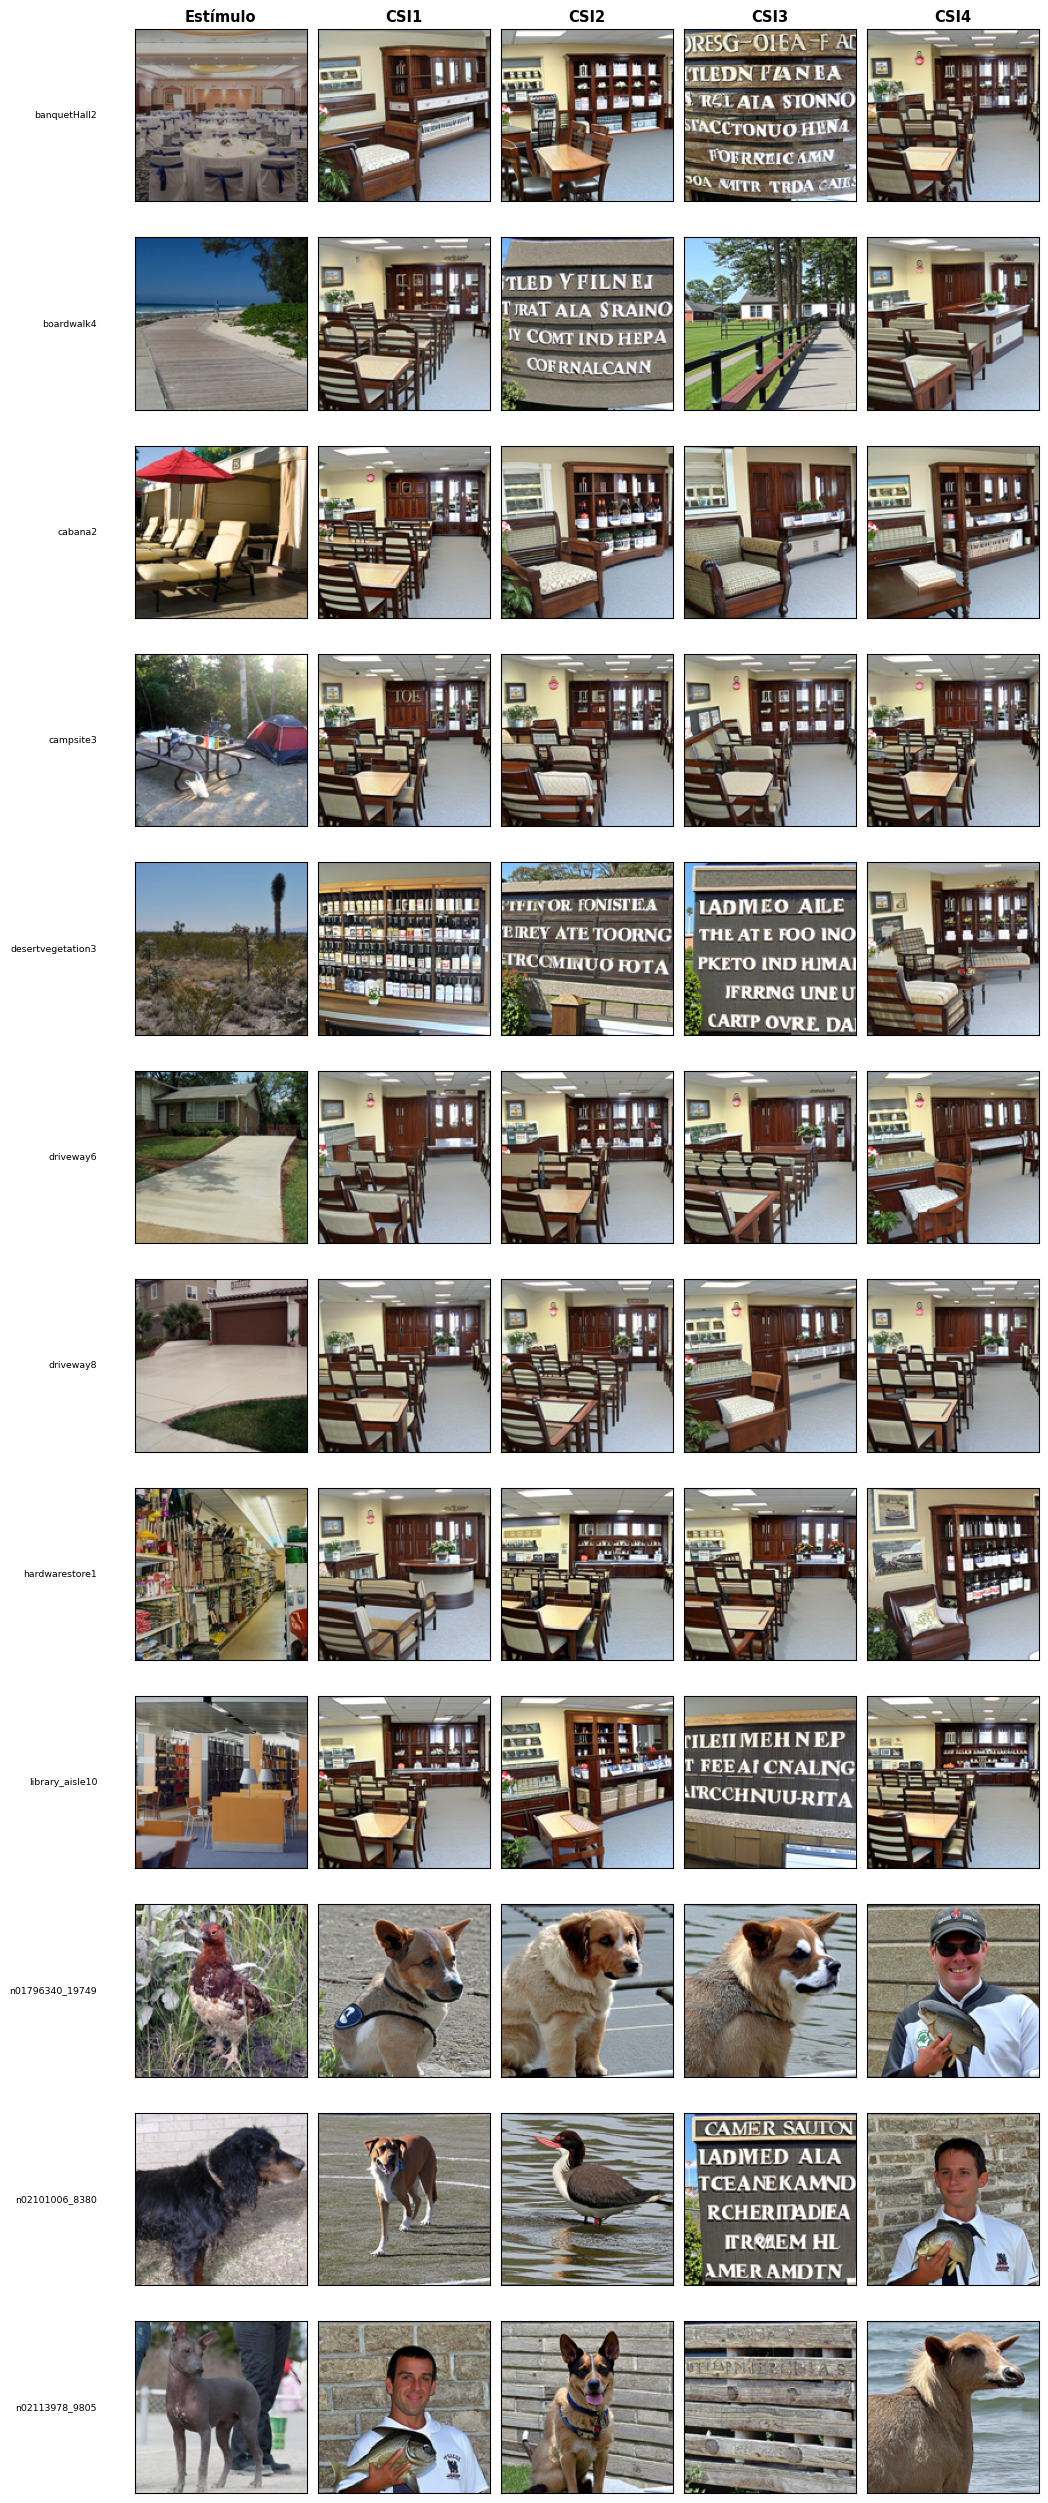
\includegraphics[width=\linewidth]{Figures/reconstrucciones/apendice/apendiceB_galeria_p03.png}
  \end{minipage}  \hfill
  \begin{minipage}[t]{0.49\textwidth}
    \centering
    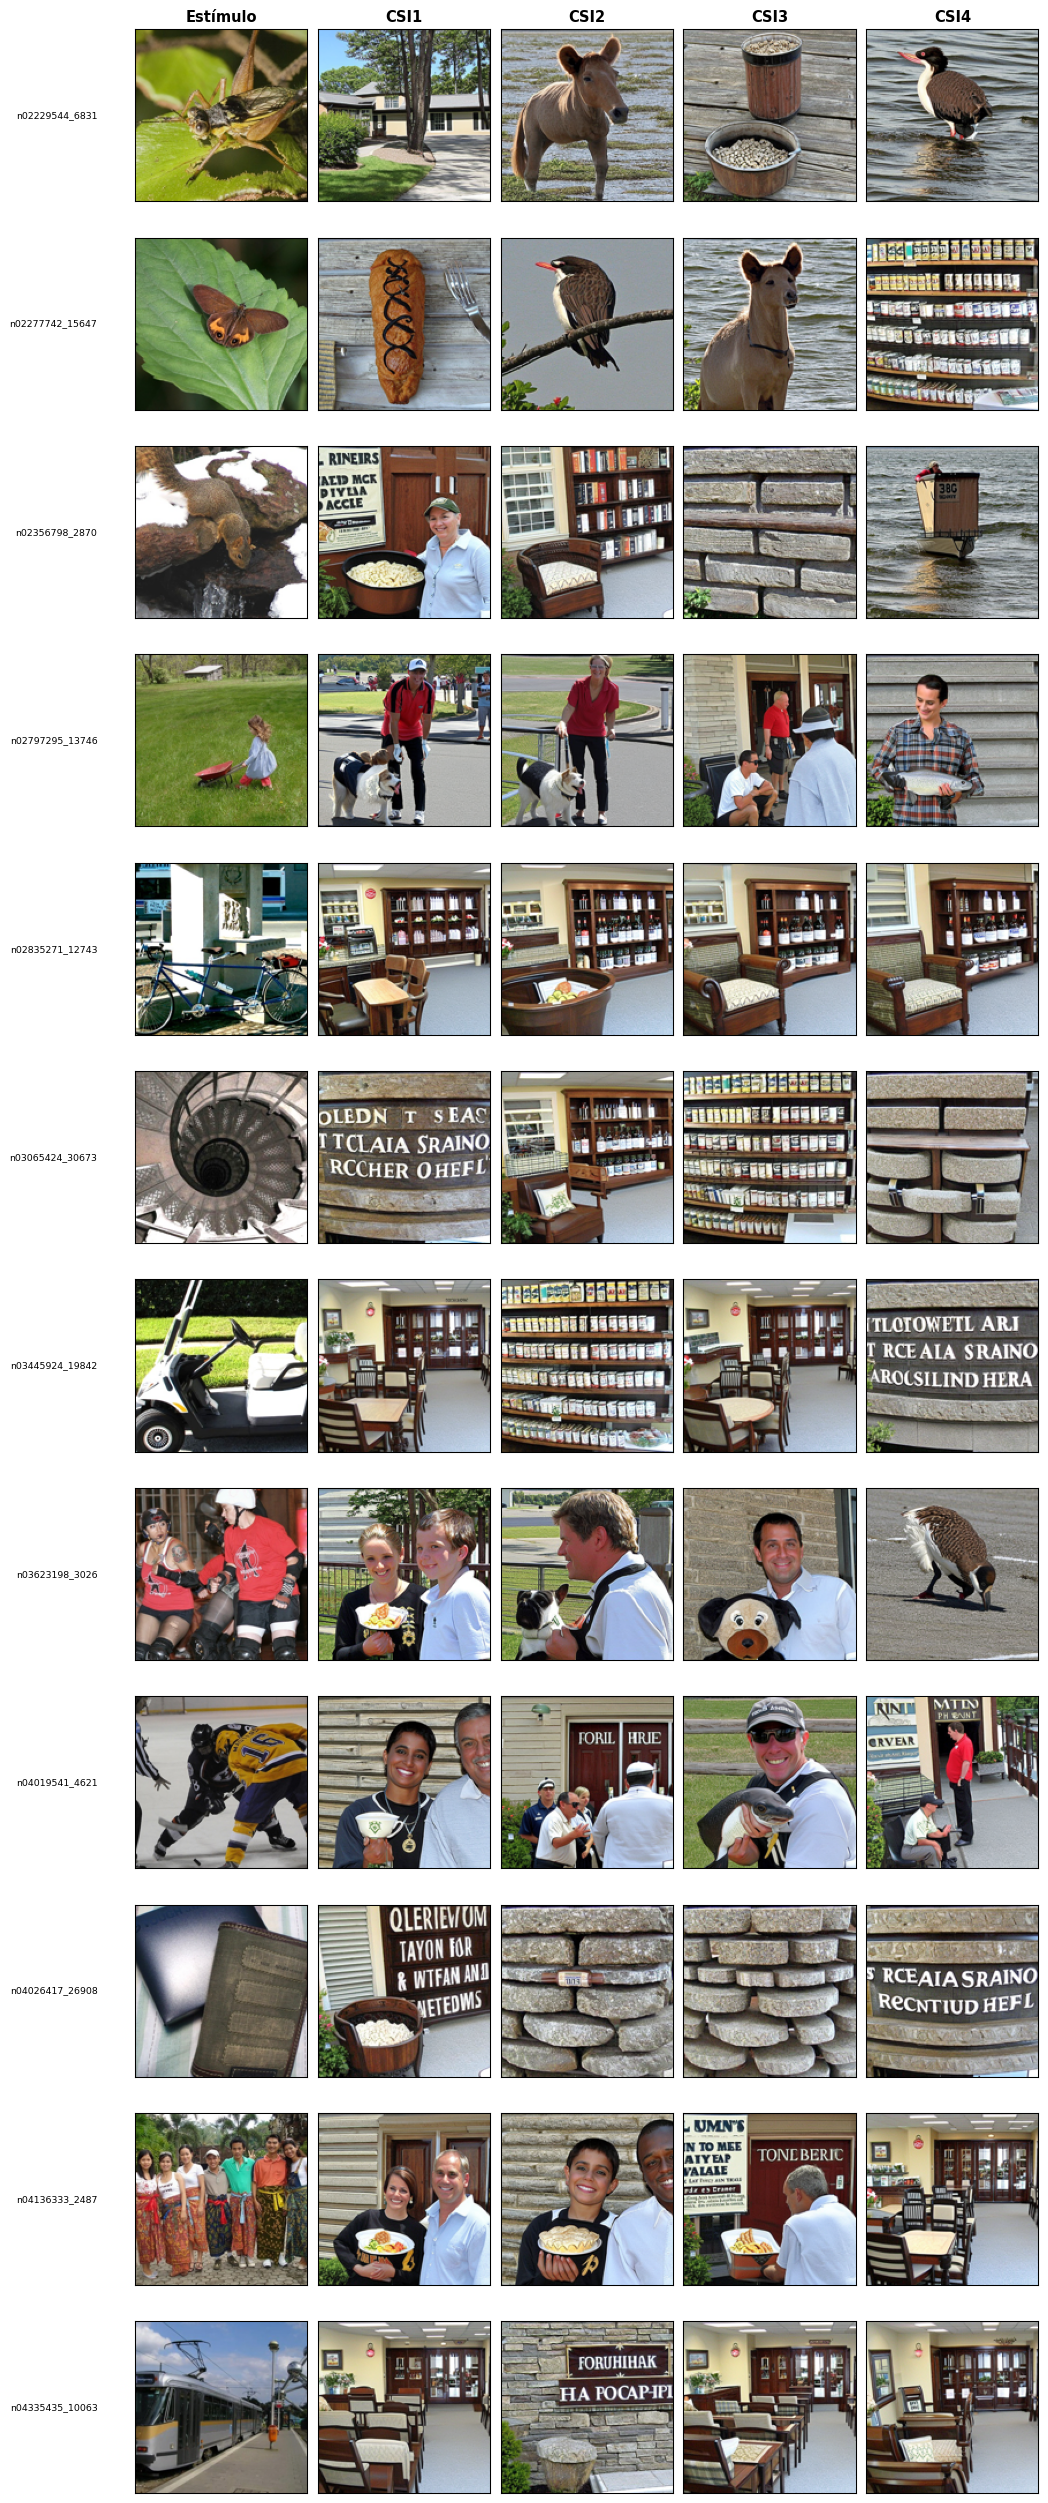
\includegraphics[width=\linewidth]{Figures/reconstrucciones/apendice/apendiceB_galeria_p04.png}
  \end{minipage}
  \caption[Galería de reconstrucciones (partes 3--4/5)]{Reconstrucciones cross-subject sobre estímulos BOLD5000 (partes 3--4 de 5). Columna~1: estímulo original; columnas~2--5: reconstrucción SD~2.1 unCLIP por sujeto (CSI1, CSI2, CSI3, CSI4).}
  \label{fig:apendiceB_galeria:g02}
\end{figure}
\clearpage

\begin{figure}[htbp]
  \centering
  \begin{minipage}[t]{0.49\textwidth}
    \centering
    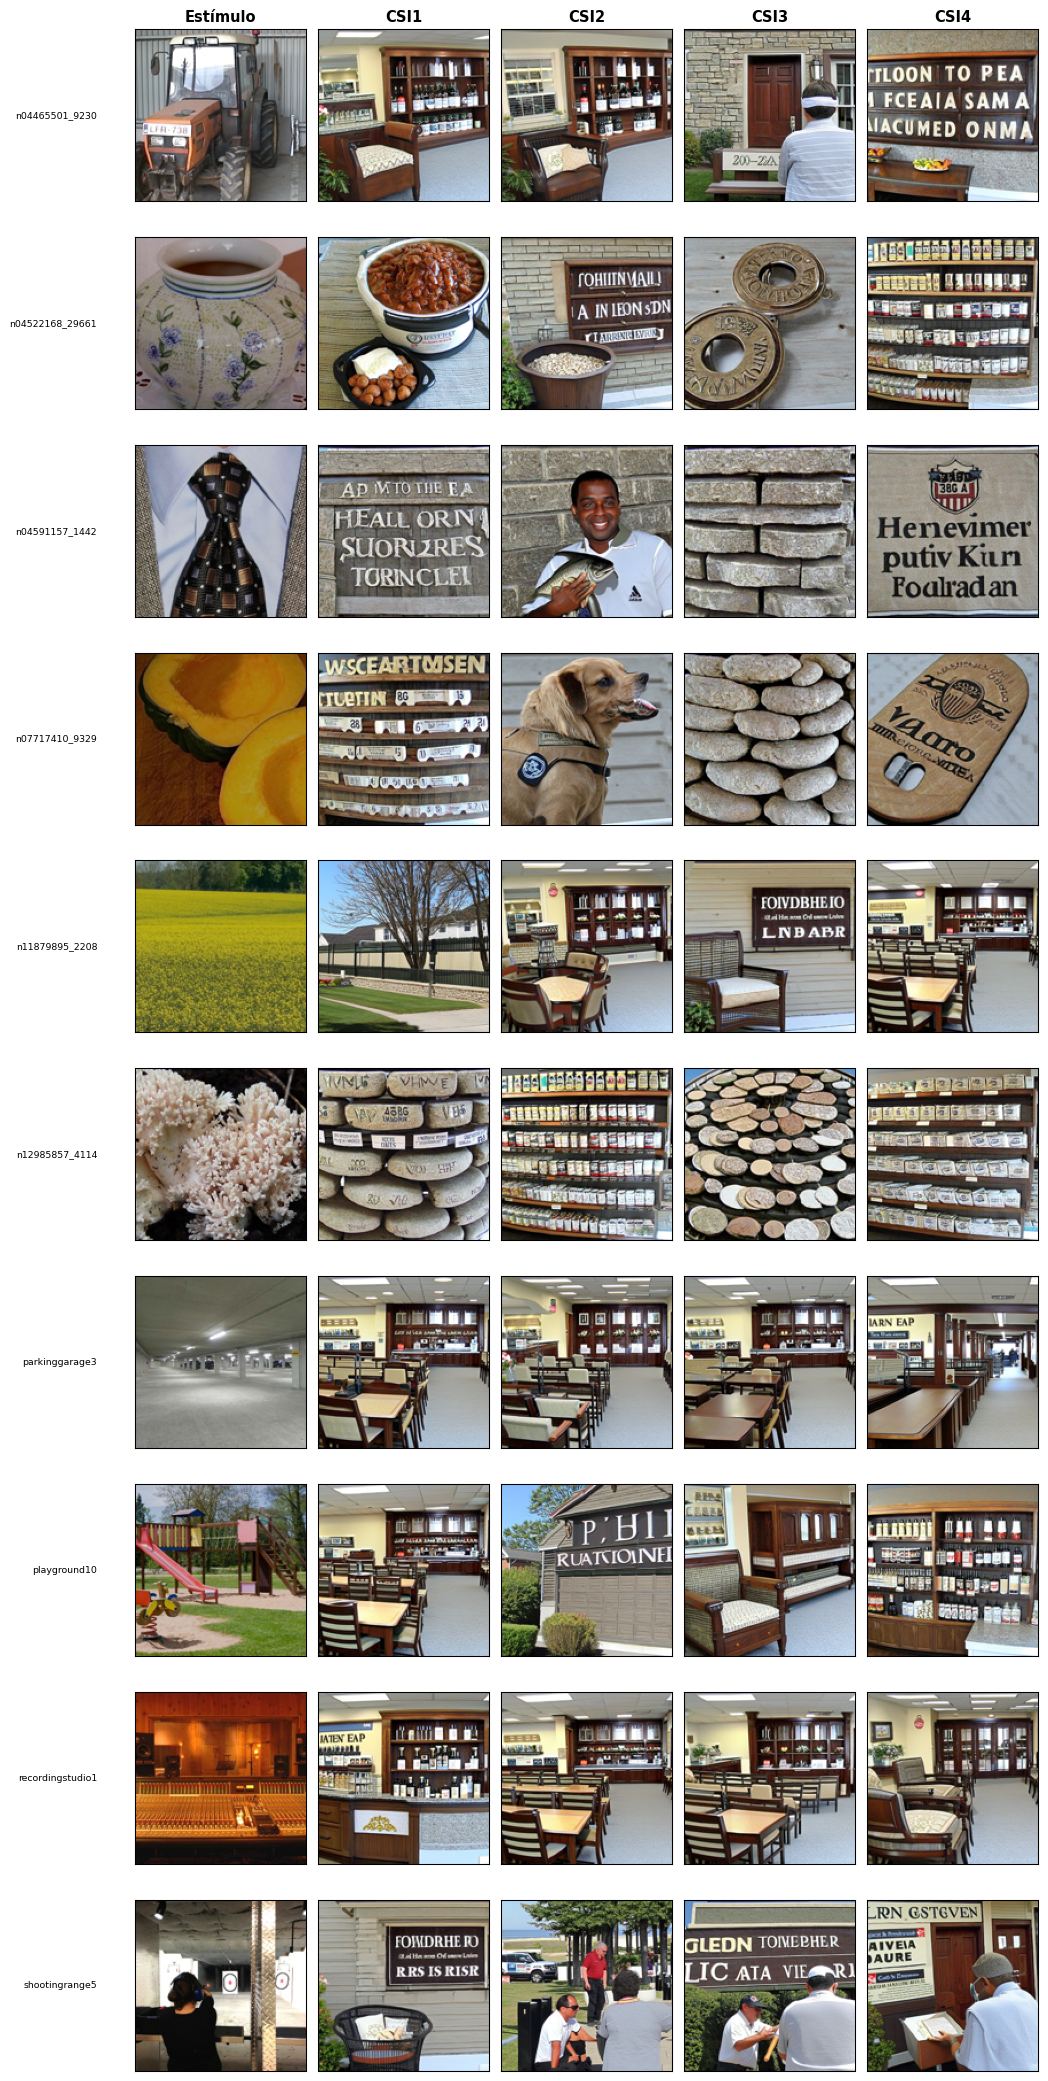
\includegraphics[width=\linewidth]{Figures/reconstrucciones/apendice/apendiceB_galeria_p05.png}
  \end{minipage}
  \caption[Galería de reconstrucciones (parte 5/5)]{Reconstrucciones cross-subject sobre estímulos BOLD5000 (parte 5 de 5). Columna~1: estímulo original; columnas~2--5: reconstrucción SD~2.1 unCLIP por sujeto (CSI1, CSI2, CSI3, CSI4).}
  \label{fig:apendiceB_galeria:g03}
\end{figure}
\clearpage
